\chapter{Конструкторский раздел}
\section{Алгоритм построения запроса в PostgreSQL}
В аналитическом разделе была рассмотрена работа планировщика запросов на верхнем уровне. Теперь же стоит заглянуть более детально в каждый из разделов и выяснить, как обрабатывается запрос, содержащий простые операторы SELECT, FROM, WHERE. Алгоритм построения запроса в PostgreSQL представлен следующим образом: на \newline рисунке \ref{image:dfd_level_0} рассмотрен верхнеуровневый процесс, рисунок  \ref{image:dfd_level_1} -- более подробно описаны шаги выполнения, необходимы для основного анализа; рисунок \ref{image:dfd_level_2} отражает этапы создания основного плана запроса; рисунок \ref{image:dfd_level_3} -- представляет непосредственно базисные функции для выбора оптимального пути \cite{source_code_postgresql, help_understanding_code}.

\begin{figure}[H]
	\centering{
		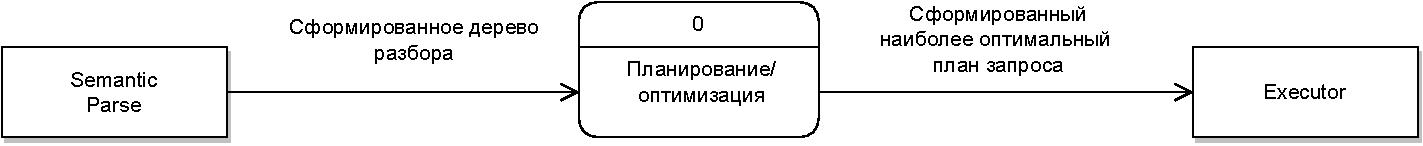
\includegraphics[scale=0.72]{./images/dfd_level_0.pdf}
		\caption{Выполнение запроса в PostgreSQL (Верхний уровень).}
		\label{image:dfd_level_0}
	}
\end{figure}

\begin{figure}[htb]
	\hfill
	\rotatebox{90}{%
		\begin{minipage}{1.6\linewidth}
			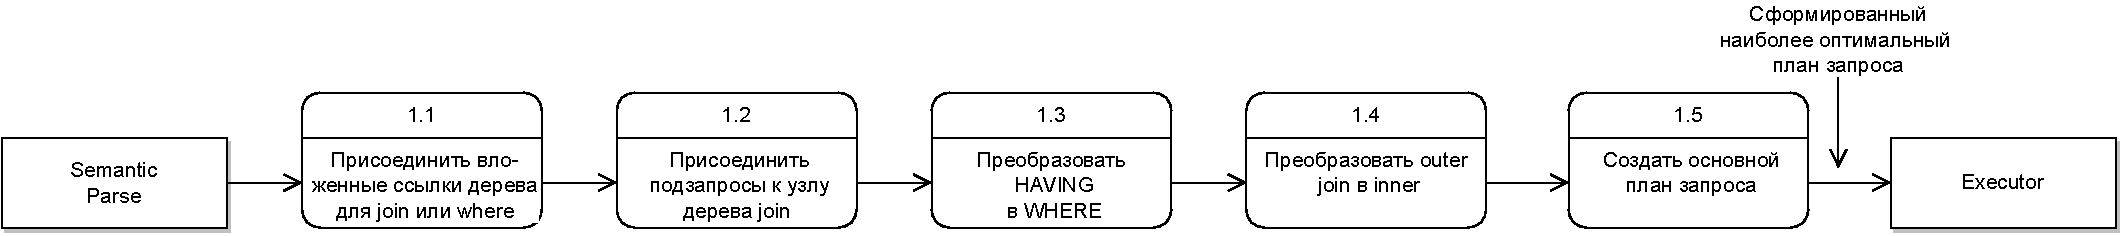
\includegraphics[width=\linewidth]{images/dfd_level_1}
			\caption{Внутренне шаги plan/optimizer}
			\label{image:dfd_level_1}
		\end{minipage}
	}\hfill
	\rotatebox{90}{%
		\begin{minipage}{1.6\linewidth}
			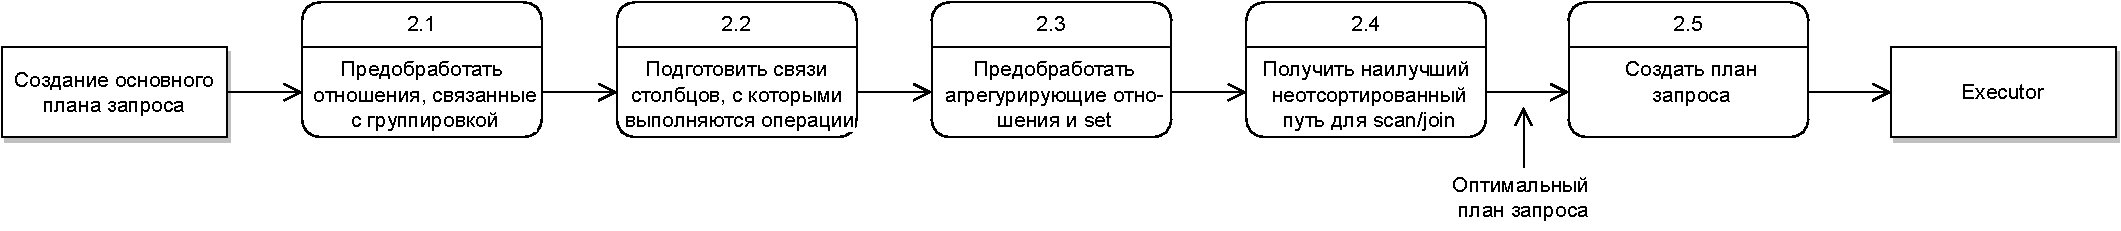
\includegraphics[width=\linewidth]{images/dfd_level_2}
			\caption{Обработка процессом 1.5}
			\label{image:dfd_level_2}
		\end{minipage}
	}\hfill\strut
	\rotatebox{90}{%
		\begin{minipage}{1.4\linewidth}
			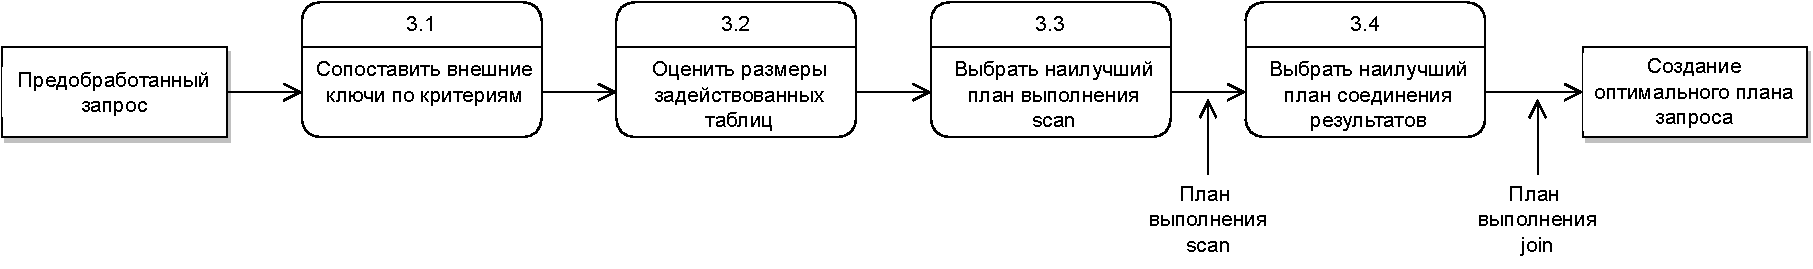
\includegraphics[width=\linewidth]{images/dfd_level_3}
			\caption{Обработка процессом 1.5}
			\label{image:dfd_level_3}
		\end{minipage}
	}\hfill\strut
\end{figure}